\documentclass[../ZF_Wing.tex]{subfiles}

\begin{document}

\subsection{Distribution}
\begin{multicols}{2}
\textbf{Hauptaufgaben\\}
\begin{itemize}
	\item \colorbox{pink!30}{Festlegung der Distributionsorgane}
	\item Festlegung des Absatzweges
	\item \colorbox{blue!30}{Festlegung der physischen Distribution}
\end{itemize}

\columnbreak

\textbf{Fragen\\}
\begin{itemize}
	\item \colorbox{pink!30}{Wer soll die Produkte verteilen?}
	\item Auf welchem Weg sollen die Produkte zum Kunden gelangen?
	\item \colorbox{blue!30}{Soll der Transport selbst oder durch einen Dritten ausgeführt werden? Welche Transportmittel sollen gewählt werden?}
\end{itemize}




\end{multicols}

\pagebreak


\subsubsection{Distributionsorgane}
\title \textcolor {teal}{UnternehmensINtern}
\begin{multicols}{3}
\textbf{Distributionsorgan\\}
\begin{itemize}
	\item Mitglieder der Geschäftsleitung
	\item Verkäufer, Aussendienstpersonal
	\item Verkaufsniederlassung
\end{itemize}

\columnbreak

\textbf{Erklärung\\}
\begin{itemize}
	\item Geschäftsleitung hat einen persönlichen Kontakt zu Grosskunden und stellt diesen selbst die neusten Produkte oder Dienstleistungen vor.
	\item Vom Unternehmen angestellt und dessen Reglen und Pflichten unterworfen. Besuchen Kunden regelmässig. Beziehen festen Lohn und z.T umsatzabhängige Provision.
	\item Vorallem von Grossunternehmen gewählt. Eigene Niederlassungen gegründet und geführt. Kundenberatungen, Verkaufsabschlüsse und Auslieferung aus eigenen Lagern.
\end{itemize}

\columnbreak

\textbf{Beispiele\\}
\begin{itemize}
	\item Textil- und Bekleidungsindustrie
	\item Versicherungen, Tupperware
	\item Modebranche, Dienstleistungssektor
\end{itemize}




\end{multicols}

\pagebreak

\title \textcolor {teal}{UnternehmensEXtern}
\begin{multicols*}{3}
\textbf{Distributionsorgan\\}
\begin{itemize}
	\item Handelsvertreter
	\item Makler
	\item Einzelhandel
	\item Grosshandel
\end{itemize}

\columnbreak

\textbf{Erklärung\\}
\begin{itemize}
	\item Selbständiger Gewerbetreibender. Produkte gehen nicht in das Eigentum des Handelsvertreters über. Vergütung umsatzorientiert.
	\item Suchen Käufer und Verkäufer von bestimmten Produkten.Bieten gegen eine Provision die Gelegenheit zum Abschluss von Geschäften an.
	\item Kauft Güter und verkauft i.d.R. ohne zusätzliche Bearbeitung an den Endkunden.
	\item Waren in grossen Mengen eingekauft und an Wiederverkäufer weiterverkauft.
\end{itemize}

\columnbreak

\textbf{Beispiele\\}
\begin{itemize}
	\item Papeteriebranche
	\item Grundstückverkäufe, Versicherungen, Bankgeschäfte
	\item Warenhaus, Bijouterie
	\item Cash and Carry
\end{itemize}

\end{multicols*}


\subsubsection{Absatzwege}

\title{\textbf{Direkte und indirekte Absatzwege: \\}}
\begin{figure}[H]
\centering
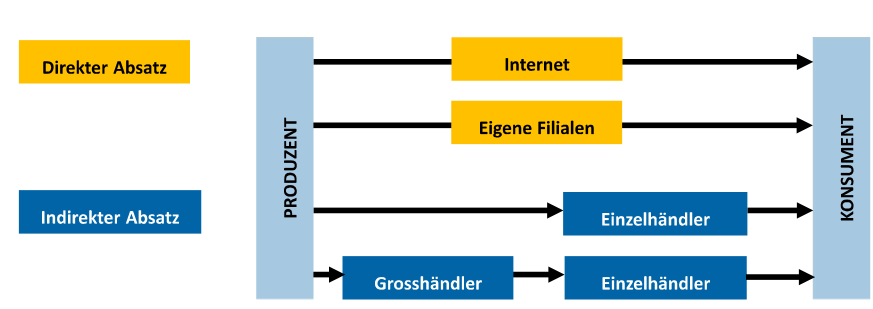
\includegraphics[width=0.3\textwidth]{Resources/Image/Absatzwege.png}
\caption{\label{fig:Absatzwege}Absatzwege.}
\end{figure}

\begin{multicols}{2}

\begin{figure}[H]
\centering
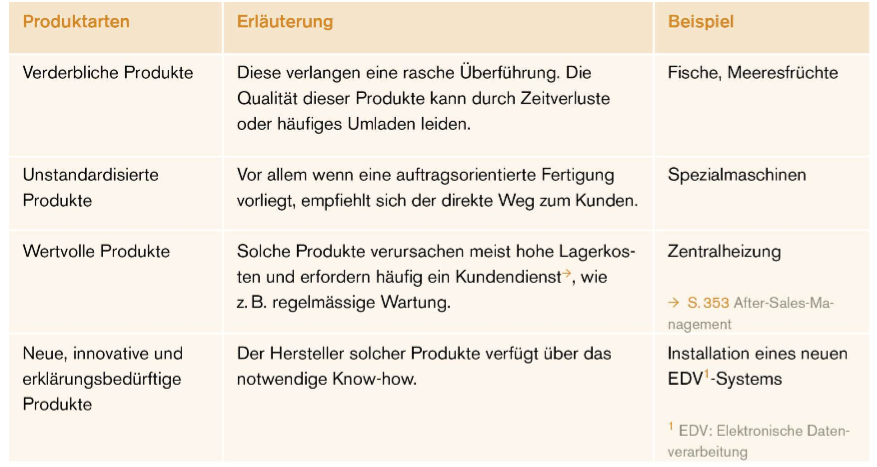
\includegraphics[width=0.3\textwidth]{Resources/Image/DirekterAbsatzweg.png}
\caption{\label{fig:DirekterAbsatzwe}DirekterAbsatzweg.}
\end{figure}


\columnbreak

\begin{figure}[H]
\centering
\includegraphics[width=0.3\textwidth]{Resources/Image/IndirekterAbsatzweg.png}
\caption{\label{fig:IndirekterAbsatzweg}IndirekterAbsatzweg.}
\end{figure}

\end{multicols}


\subsection{Kommunikation}

\begin{itemize}
	\item Werbung
	\begin{itemize}
		\item Gedruckte Anzeigen
		\item Radiowerbung
		\item Kino- und TV-Werbung
		\item Kataloge
		\item Plakaten
		\item Internet
	\end{itemize}
	\item Public Relations (PR)
	\begin{itemize}
		\item Unternehmensleitbild
		\item Betriebsbesichtigungen
		\item Jahresberichte
		\item Spenden
		\item Medienkontakte
	\end{itemize}
	\item Sponsoring
	\begin{itemize}
		\item Sportsponsoring
		\item Wissenschaftsponsoring etc.
	\end{itemize}
	\item Verkaufsförderung
	\begin{itemize}
		\item Prämien
		\item Warenproben etc.
	\end{itemize}
	\item Persönlicher Verkauf
	\begin{itemize}
		\item Product Placement
	\end{itemize}
\end{itemize}


\subsubsection{Kommunikationsinstrumente}
Marketing $\neq$ Promotion $\neq$ Public Relations

\textbf{Marketing\\}
\begin{itemize}
	\item 4P'S
	\begin{itemize}
		\item Ziele
		\begin{itemize}
			\item Umsatz
			\item Marktanteile
			\item Deckungsbeiträge
		\end{itemize}
	\end{itemize}
\end{itemize}



\textbf{Public Relations\\}
\begin{itemize}
	\item Zielgerichtete Darstellung einer Organisation und deren Anliegen bei ihren relevanten Dialoggruppen.
	\begin{itemize}
		\item Ziele
		\begin{itemize}
			\item Image
			\item Vertrauen
			\item Reputation
			\item Wissen
			\item Akzeptanz
		\end{itemize}
	\end{itemize}
\end{itemize}


\subsubsection{Vermarktungsobjekte}

\begin{enumerate}
	\item Konsumgüter-Marketing
	\item Investitionsgüter-Marketing
	\item Dienstleistungs-Marketing
	\item Non-Profit-Marketing
	\item Social Marketing
	\item Destination Marketing
	\item Handels-Marketing
\end{enumerate}


\subsubsection{Wie funktioniert Werbung?}

\textbf Attention \\
\textbf Interest \\
\textbf Desire \\
\textbf Action \\

= AIDA Formel

\paragraph{Custom Decision Journey}
\begin{multicols}{2}

\title{Lineares Stufenmodell}

\begin{figure}[H]
\centering
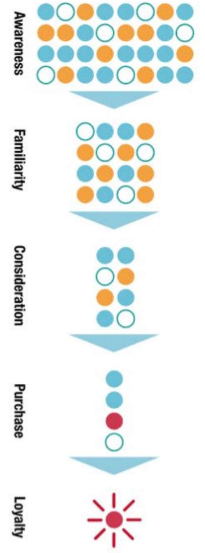
\includegraphics[width=0.3\textwidth]{Resources/Image/LinearesStufenmodell.png}
\caption{\label{fig:LinearesStufenmodell}LinearesStufenmodell.}
\end{figure}

\columnbreak

\begin{figure}[H]
\centering
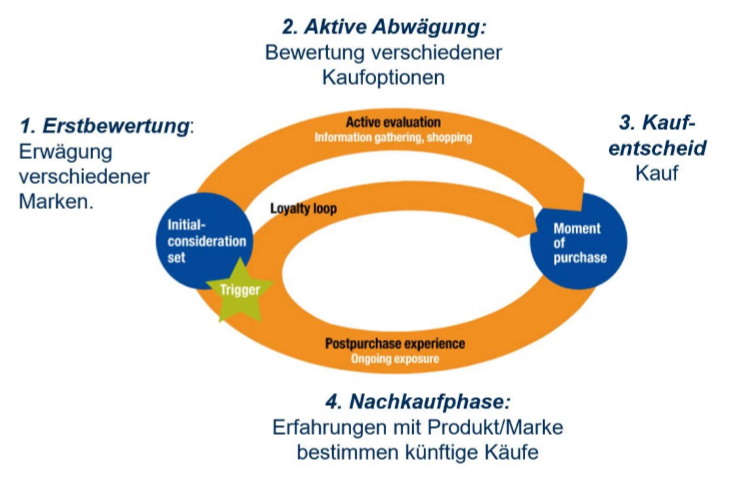
\includegraphics[width=0.3\textwidth]{Resources/Image/CustomDecisionJourney.png}
\caption{\label{fig:CustomDecisionJourney}CustomDecisionJourney.}
\end{figure}

\end{multicols}


\textbf{Werbung Ziele\\}

\begin{itemize}
	\item Umsatz
	\item Bekanntheit
	\item Wissen
	\item Einstellungen, Images
\end{itemize}

\begin{multicols}{2}
\textbf{Inhalte eines Konzeptes}

\begin{itemize}
	\item Werbeobjekt (Produkt)
	\item Werbesubjekt (Zielgruppe)
	\item Wirkungsziele
	\item Werbebotschaft
	\item Werbemittel
	\item Werbeperiode
	\item Werbebudget
\end{itemize}

\columnbreak

\textbf{Botschafen und Botschafter}
\begin{enumerate}
	\item Lifestyle-Technik
	\item Slice-of-Life-Technik
	\item Dreamworld-Technik
	\item Stimmungs-Gefühlsbilder
	\item Persönlichkeit als Symbolfigur
	\item Technische Kompetenz
	\item Wissenschaftlicher Nachweis
	\item Testimonial-Werbung
	\item Influecer
\end{enumerate}




\end{multicols}

\begin{multicols}{2}

\begin{figure}[H]

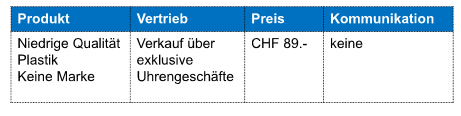
\includegraphics[width=0.3\textwidth]{Resources/Image/HarmonischeMarketingMix1.png}
\caption{\label{fig:HarmonischeMarketingMix1}HarmonischeMarketingMix1.}
\end{figure}

\columnbreak

\begin{figure}[H]

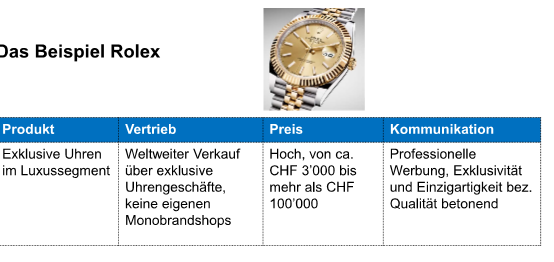
\includegraphics[width=0.3\textwidth]{Resources/Image/HarmonischerMarketingMix2.png}
\caption{\label{fig:HarmonischerMarketingMix2}HarmonischerMarketingMix2.}
\end{figure}


\end{multicols}


\subsection{Markenführung}


\subsubsection{Aspekte}
\begin{itemize}
	\item Weckt Assoziationen
	\item Nutzen
	\item Werte
	\item Persönlichkeit und Nutzeridentifizierung
\end{itemize}



\subsubsection{Signalfunktion}

\begin{itemize}
	\item Qualität
	\item Preis
	\item Funktionalität
	\item Emotionen
\end{itemize}



\subsubsection{Markenwert}

Zur Ermittlung in 7 Bereiche aufgeteilt: \\

\begin{enumerate}
	\item Dynamik
	\item Stabilität
	\item Marktführerschaft
	\item Entwicklung
	\item Kontinuität
	\item Internationalisierungsgrad
	\item Markenschutz
\end{enumerate}

\textbf{Definition: } Present Value der künftigen Erträge, die mit der Marke erwirtschaftet werden.\\

\paragraph{Formen der Verknüpfung: \\}

\begin{itemize}
	\item Einzelproduktmarken/Monomarken (Ariel, Bounty)
	\item Sortimentmarke (BMW)
	\item Mehrere Sortimentsmarken (Nivea)
	\item Mehrschichtige Markenverknüfpungen (VW, Audi, Bentley....)
\end{itemize}



\subsection{Customer Relationship Management (CRM)}
\textbf{Ziel: } Kundengewinnung + Kundenbindung\\
Kundengewinnung ist 5x teurer, als die Bindung von Kunden!\\

\paragraph{Aufgaben der Kundenbindung: \\}
\begin{itemize}
	\item Kundenpotential erhalten
	\begin{itemize}
		\item Kontinuierliche Wiederkäufe erzeugen
		\item Beschwerdemanagement
		\item After-Sales-Management 
	\end{itemize}
	\item Kuntenpotential ausbauen
	\begin{itemize}
		\item Zusatzkäufe erzeugen/erhöhen
		\item Folgekäufe erzeugen/erhöhen
		\item Wiederkäufe erhöhen (Menge,Art,Preis)
	\end{itemize}
\end{itemize}


\subsubsection{CRM Instrumente}

\title{Produktpolitik}
\begin{table} [H]

\begin{tabular}{l}

\colorbox{pink!30}{\textbf{Massnahmen mit dem Fokus " Interaktion"} }

\\\hline
- Gemeinsame Produktentwicklung\\
\hline
\colorbox{pink!30}{\textbf{Massnahmen mit dem Fokus "Zufriedenheit"}}\\
\hline
- Individuelle Angebote\\
- Qualitätsstandards\\
- Servicestandards\\
- Zusatzleistungen\\
- Garantien\\
\hline
\colorbox{pink!30}{\textbf{Massnahmen mit dem Fokus " Wechselbarriere"}}\\
\hline
- individuelle technische Standards\\
\end{tabular}
\end{table}



\title{Preispolitik}
\begin{table} [H]

\begin{tabular}{l}

\colorbox{pink!30}{\textbf{Massnahmen mit dem Fokus " Interaktion"} }

\\\hline
- Kundenkarten\\
\hline
\colorbox{pink!30}{\textbf{Massnahmen mit dem Fokus "Zufriedenheit"}}\\
\hline
- Preisgarantien\\
- Zufriedenheitsabhängige Preisgestaltung\\
\hline
\colorbox{pink!30}{\textbf{Massnahmen mit dem Fokus " Wechselbarriere"}}\\
\hline
- Rabatt- und Bonussysteme\\
- Prisdifferenzierung\\
- Kundenkarten\\
\end{tabular}
\end{table}

\title{Distributionspolitik}
\begin{table} [H]

\begin{tabular}{l}

\colorbox{pink!30}{\textbf{Massnahmen mit dem Fokus " Interaktion"} }

\\\hline
- Kundenbesuche\\
\hline
\colorbox{pink!30}{\textbf{Massnahmen mit dem Fokus "Zufriedenheit"}}\\
\hline
- Online-Bestellung\\
- Katalogverkauf\\
- Direktverkauf\\
\hline
\colorbox{pink!30}{\textbf{Massnahmen mit dem Fokus " Wechselbarriere"}}\\
\hline
- Abonnemente\\
- Standortwahl
\end{tabular}
\end{table}




\title{Kommunikationspolitik}
\begin{table} [H]

\begin{tabular}{l}

\colorbox{pink!30}{\textbf{Massnahmen mit dem Fokus " Interaktion"} }

\\\hline
- Direkt-Mail\\
- Events\\
- Servicenummern\\
- Gewinnspiele\\
- Produktmuster\\
\hline
\colorbox{pink!30}{\textbf{Massnahmen mit dem Fokus " Zufriedenheit"}}\\
\hline
- Kundenclubs\\
- Kundenzeitschriften\\
- Beschwerdemanagement\\
\hline
\colorbox{pink!30}{\textbf{Massnahmen mit dem Fokus " Wechselbarriere"}}\\
\hline
- Rabatt- und Bonussysteme\\
- Prisdifferenzierung\\
- Kundenkarten\\
\end{tabular}
\end{table}

\title{Kundenpotential ausbauen \\}
\begin{itemize}
	\item Wiederverkäufe erhöhen (Wechsel Rasierermodell Gillette Mach 3 Turbo z Mach 3 Power)
	\item Folgekäufe erzeugen und/oder erhöhen (Kauf Rasierklingen v. Gillette)
	\item Zusatzkäufe erzeugen und/oder erhöhen (Aftershave von Gilette)
\end{itemize}


















































\end{document}